\documentclass[pagenumber=off]{article}

\usepackage[pdftex]{graphicx}
\usepackage{xcolor}
\usepackage[a4paper,margin=0.7in,portrait]{geometry}
\usepackage{etoolbox}

%----------------------------------------------------------
\definecolor{coolblack}{rgb}{0.0, 0.18, 0.39}
%\AtBeginDocument{\color{coolblack}}
%----------------------------------------------------------

%%----------------------------------
\begin{document}

%%--- Title ---
\begin{titlepage}
\begin{center}
\vspace{1cm}
{\textcolor{gray}\today}\\
{\textcolor{gray}{\bf Udacity Nanodegree: Deep Reinforcement Learning }}\\
\vspace{1.5cm}
{\textcolor{coolblack}{\huge \bf DRL Project 1: Navigation}}\\
\vspace{0.5cm}
{\textcolor{coolblack}{\Large \bf  Train a Deep Q-Learning Agent}}
\par
\vspace{0.5cm}
{\textcolor{coolblack}{\Large\itshape Solve a navigation task using a deep neural network to approximate Q-Function.}}\par
\vspace{6cm}
\end{center}
\tableofcontents

\vspace{6cm}

\begin{center}
{Alberto M. Cozzini}\\
\end{center}
\end{titlepage}

%----------------------------------
\section{Task}
For this project, an agent has to learn to navigate and collect bananas in a large, square world.\\
A reward of +1 is provided for collecting a yellow banana, and a reward of -1 is provided for collecting a blue banana.\\
The goal of the agent is to collect as many yellow bananas as possible while avoiding blue bananas. The task is episodic and in order to solve the environment the agent must get an average score of at least +13 over 100 consecutive episodes.


%----------------------------------
\begin{figure}[!h]
  \centerline{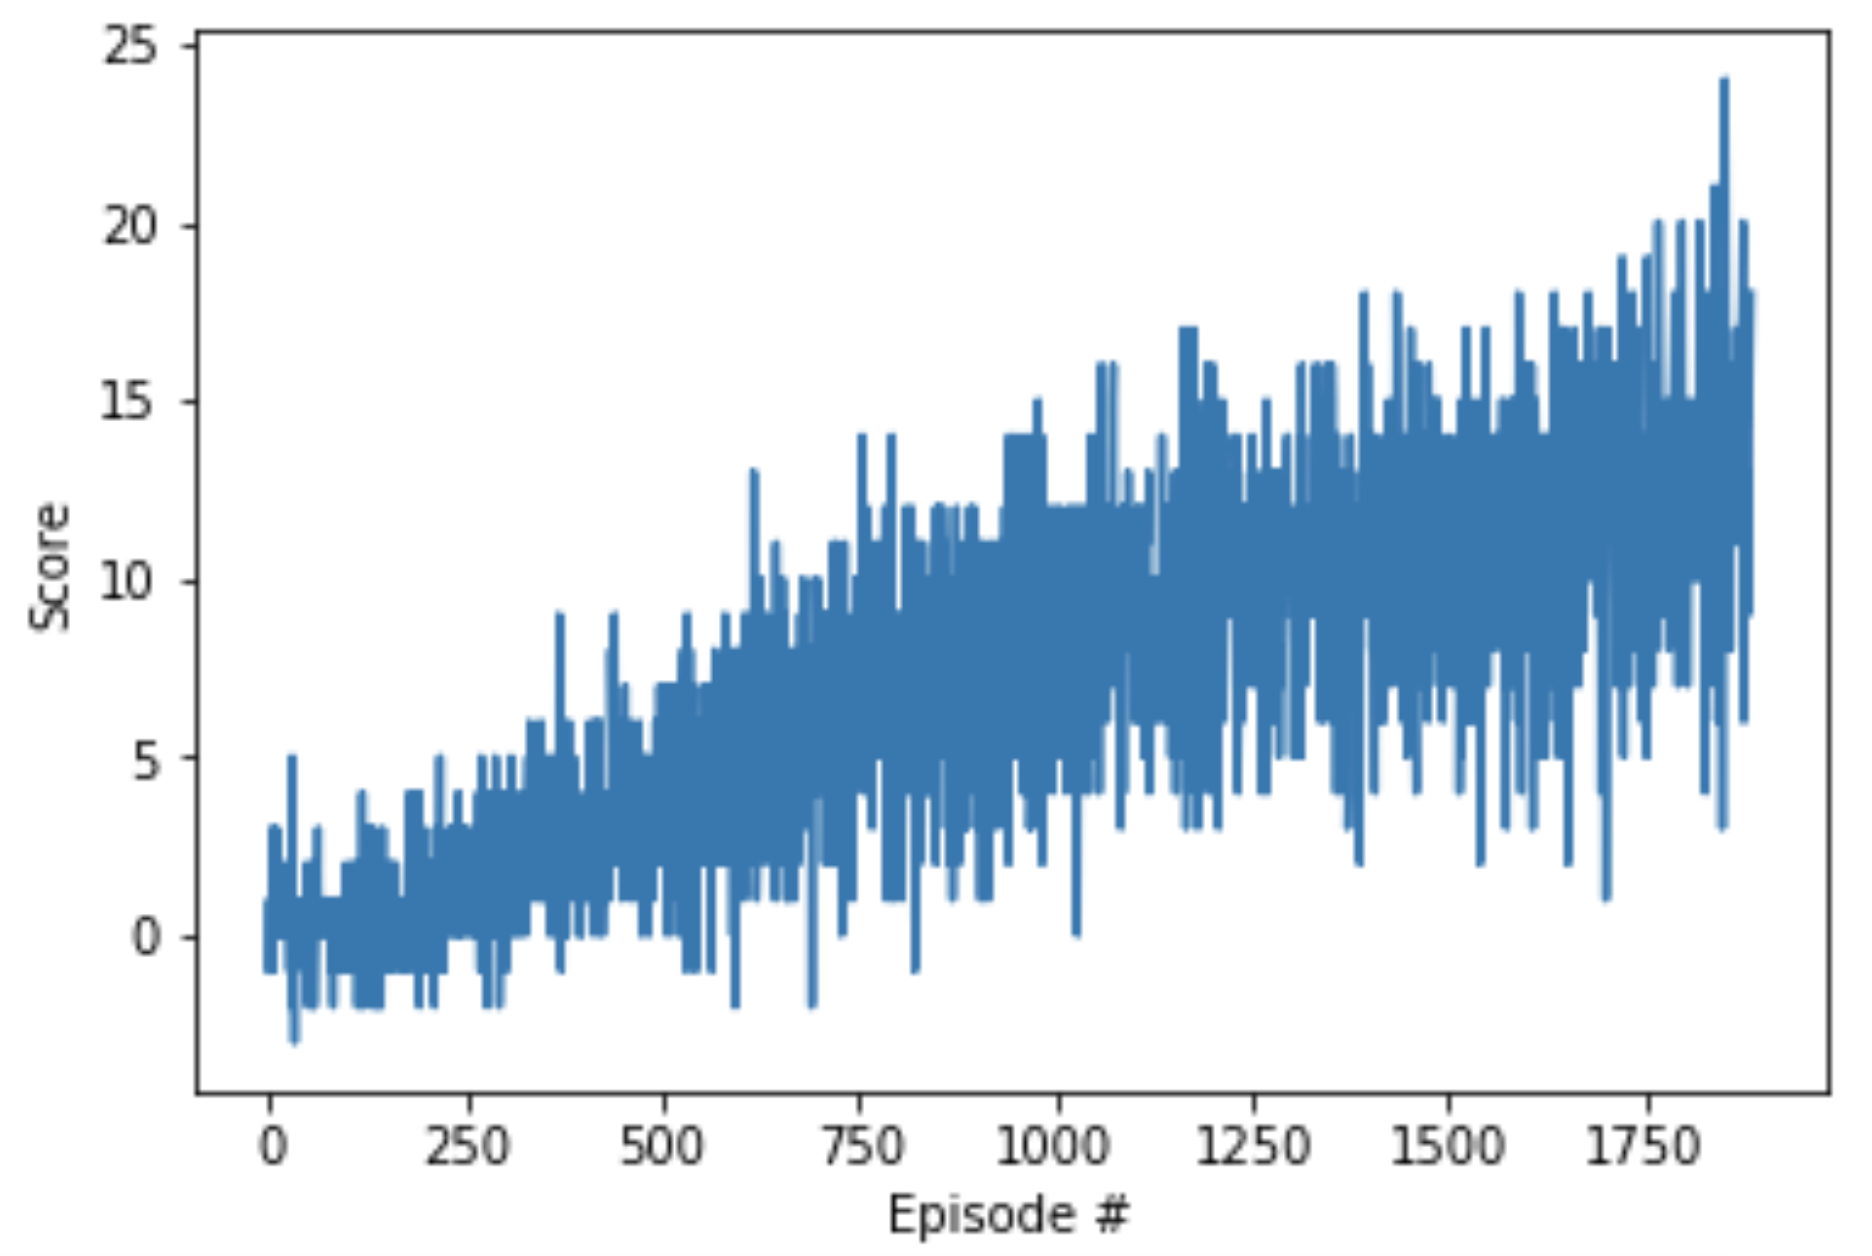
\includegraphics[page=1, height=6cm, width=12 cm, angle=0]{./Benchmark_Score.png}}
  \caption{Benchmark Implementation. It reaches an average score of at least 13 after about 1800 episodes.}
\end{figure}

%----------------------------------


%----------------------------------
\section{Environment}
The environment is built on Unity architecture.\\
The state space has 37 dimensions and contains the agent's velocity, along with ray-based perception of objects around agent's forward direction. Given this information, the agent has to learn how to best select actions. Four discrete actions are available, corresponding to: 0 move forward, 1 move backward, 2 turn left, 3 turn right.


%----------------------------------
\section{Model}


\subsection{Agent}

The agent objective is to learn by interacting with the environment.\\
The utility function of the agent values the immediate reward more than the futures rewards which are discounted at a factor of 0.99 per time step.


\subsubsection{{\Large $\epsilon$}-Greedy Policy}

The agent learns following an Epsilon-Greedy policy with respect the action-value Q function.
At the beginning of the learning process it is prone to explore with probability 1, $\epsilon$.
Subsequently the $\epsilon$ decays at a rate of 0.995 till it reaches a floor of 0.01.


\subsubsection{Soft Update}

One method we adopt to improve stability of learning process and avoid oscillations or divergence of the policy, is to use a separate network to generate target Qs values. While the two networks are identical clones, we only update the weights of the target network periodically after every batch of experiences.

To smooth the update even further the new targets weights are updated by interpolating old with new local weights with a factor of 0.001.

\subsubsection{Experience Replay}

To make the learning process more stable and avoid aberration of the action-value Q function, we store and randomly replay some of the recent experiences.

The number of experiences we store in hour memory is 1e5. Each time we sample uniformly at random a batch of 64.


\subsection{Q Network}

The inputs are the 37 state variables whereas the outputs correspond to the predicted Q value for each action given the input state.
The network has three hidden layers of fully connected nodes. The first layer has 150 rectifier units, the second 120 and the third 60. The output layer is a fully-connected linear layer with a single output for each valid action. 



\subsection{Loss Function}

Following the Bellman equation, the loss function is the mean square error between the expected Q values computed on the local network and the target Q values computed on the network the momentarily older frozen weights.  

\subsubsection{Optimizer}

The optimizer performs a stochastic gradient descent step on the loss function with respect to the network weights.\\
We implement the Adam optimization algorithm with learning rate of 0.0005.\\
For more information see {\it Adam: A Method for Stochastic Optimization}.



%\newpage
%----------------------------------
\section{Results}

After less then 700 training episodes it reaches an average score of more than 15..  

\begin{table}[h]
  \centering
    \begin{tabular}{|l|c|}
      \hline
      {\bf Episode} & {\bf Average Score} \\ 
      \hline
      100 & 0.56 \\
      200 & 3.56 \\
      300 & 6.73 \\
      400 & 9.69 \\
      500 & 12.90 \\
      600 & 13.85 \\
      700 & 14.33 \\
      \hline
      {\bf 745} & {\bf 15.02} \\      
      \hline
    \end{tabular}
    \caption{Agent learning curve. Rolling average score over previous 100 episodes.}
  \end{table}

\vspace{-1cm}
%----------------------------------
\begin{figure}[!h]
  \centerline{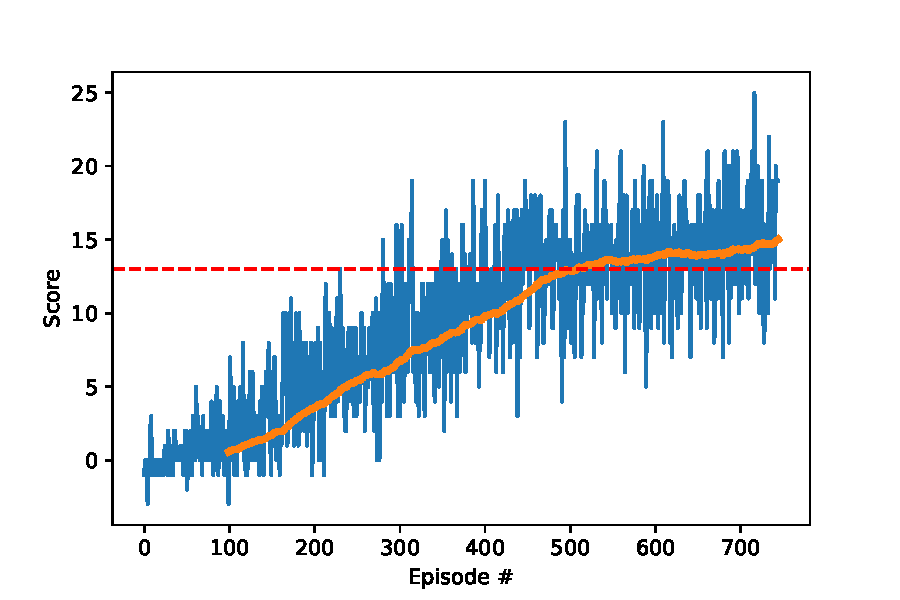
\includegraphics[page=1, height=8cm, width=14cm, angle=0]{./Average_Score.pdf}}
  \caption{Score by episode. Agent learns to identify and move towards yellow bananas.}
\end{figure}

%----------------------------------

%\newpage
%----------------------------------
\section{Future Work}

The current solution is already quite efficient in reaching its target in reasonably number of episodes.
Nonetheless, looking at possible ways to improve the current architecture one immediate route to explore would be implement prioritized experience replay. We are currently uniformly sampling from past experiences, but a likely improvement would be to prioritize samples that yielded greater weights updated, i.e. greater TD error.

\end{document}
